%done: replaced .. by \ldots
%\newcommand{\set}[1]{\{#1\}}
%\newcommand{\setcomprehension}[2]{\{#1 \mid{ } #2\}}
% TODO: fix arrows in geiger-bn
% Fix figure 1 to read ``hypothesis'' instead of ``conjecture''
% Fix Geiger example to make gender parent of type

\documentclass{elsarticle}%
%\usepackage{fullpage}
%\usepackage{times}
\usepackage{amsmath}
\usepackage{amsthm}
\usepackage{amsfonts}
\usepackage{amssymb}
\usepackage{graphicx}
\usepackage{subfigure}
\usepackage{epstopdf}%
\setcounter{MaxMatrixCols}{30}
\usepackage{todonotes}
\usepackage[normalem]{ulem}

\makeatletter
\newlength{\mySpaceUnder}
\newlength{\mySpaceOver}
% \setlength{\mySpaceUnder}{0.25cm}  % 4cm as an example ;-)
% \setlength{\mySpaceOver}{0.25cm}   % 3cm as an example
%                                    {\mySpaceOver}%
%                                    {\mySpaceUnder}%
\renewcommand\section{\@startsection {section}{1}{\z@}%
  {-12\p@ \@plus -4\p@ \@minus -4\p@}%
                       {12\p@ \@plus 4\p@ \@minus 4\p@}%
                                   {\normalfont\large\bfseries\boldmath
                                   \rightskip=\z@ \@plus 8em\pretolerance=10000 }}

\renewcommand\subsection{\@startsection {subsection}{1}{\z@}%
  {-8\p@ \@plus -4\p@ \@minus -4\p@}%
                       {8\p@ \@plus 4\p@ \@minus 4\p@}%
                                   {\normalfont\large\bfseries\boldmath
                                   \rightskip=\z@ \@plus 8em\pretolerance=10000 }}
\makeatother

%TCIDATA{OutputFilter=latex2.dll}
%TCIDATA{Version=5.00.0.2606}
%TCIDATA{CSTFile=40 LaTeX article.cst}
%TCIDATA{Created=Monday, July 24, 2006 15:29:01}
%TCIDATA{LastRevised=Thursday, January 11, 2007 11:29:24}
%TCIDATA{<META NAME="GraphicsSave" CONTENT="32">}
%TCIDATA{<META NAME="SaveForMode" CONTENT="1">}
%TCIDATA{BibliographyScheme=Manual}
%TCIDATA{<META NAME="DocumentShell" CONTENT="Standard LaTeX\Blank - Standard LaTeX Article">}
\DeclareGraphicsRule{.tif}{png}{.png}{`convert #1 `basename #1 .tif`.png}
 \newtheorem{theorem}{Theorem}
\setlength{\textfloatsep}{0pt}
\setlength{\intextsep}{11pt}
\newtheorem{assertion}[theorem]{Assertion}
\newtheorem{acknowledgement}[theorem]{Acknowledgement}
\newtheorem{algorithm}[theorem]{Algorithm}
\newtheorem{axiom}[theorem]{Axiom}
% \newtheorem{case}[theorem]{Case}
% \newtheorem{claim}[theorem]{Claim}
% \newtheorem{conclusion}[theorem]{Conclusion}
% \newtheorem{condition}[theorem]{Condition}
% \newtheorem{conjecture}[theorem]{Conjecture}
 \newtheorem{corollary}[theorem]{Corollary}
% \newtheorem{criterion}[theorem]{Criterion}
\newtheorem{definition}[theorem]{Definition}
 \newtheorem{example}[theorem]{Example}
% \newtheorem{exercise}[theorem]{Exercise}
 \newtheorem{lemma}[theorem]{Lemma}
% \newtheorem{notation}[theorem]{Notation}
% \newtheorem{problem}[theorem]{Problem}
 \newtheorem{proposition}[theorem]{Proposition}
% \newtheorem{remark}[theorem]{Remark}
% \newtheorem{solution}[theorem]{Solution}
% \newtheorem{summary}[theorem]{Summary}
\newtheorem{observation}[theorem]{Observation}
\renewenvironment{proof}[1][Proof]{\noindent\textbf{#1.} }{\ \rule{0.5em}{0.5em}}
\newenvironment{proof-outline}[1][Proof Outline]{\noindent\textbf{#1.} }{\ \rule{0.5em}{0.5em}}
\DeclareMathOperator{\content}{content}
\DeclareMathOperator{\card}{card}
\DeclareMathOperator{\Perp}{\perp{}\!\!\!\!\!\!\perp{}}
\DeclareMathOperator{\SEQ}{SEQ}
\DeclareMathOperator{\MC}{MC}
\DeclareMathOperator{\ID}{ID}
\DeclareMathOperator{\CONV}{CP}
\DeclareMathOperator{\pattern}{\pi}
\DeclareMathOperator{\Poly}{\mathbf{\mathrm{P}}}
\DeclareMathOperator{\RP}{\mathbf{\mathrm{RP}}}
\DeclareMathOperator{\FP}{\mathbf{\mathrm{FP}}}
\DeclareMathOperator{\NP}{\mathbf{\mathrm{NP}}}
\DeclareMathOperator{\E}{E}
\renewcommand{\d}{\mathbf{d}}

\newcommand{\learnera}{\Psi}
\newcommand{\learnerb}{\Phi}
\newcommand{\occam}{\learnera_{\mathit{occam}}}

\newcommand{\true}{\mathit{T}}
\newcommand{\false}{\mathit{F}}
\newcommand{\ZZ}{\mathbf{Z}}
\DeclareMathOperator{\sets}{sets}
\DeclareMathOperator{\Set}{set}
\DeclareMathOperator{\member}{member}
\DeclareMathOperator{\Par}{Par}
\DeclareMathOperator{\eff}{eff}
\newcommand{\set}[1]{\mathbf{#1}}
%\newcommand{\list}[1]{\mathbf{#1}}
\newcommand{\setcomprehension}[2]{\{#1:#2\}}
\newcommand{\indep}{\ensuremath{\perp{}\!\!\!\!\!\!\!\perp{}}}
\newcommand{\dep}{\ensuremath{{\perp{}\!\!\!\!\!\!\!\not  \perp{}}}}
\renewcommand{\L}{\mathcal{L}}
\newcommand{\hypothesis}{H}
\newcommand{\hypotheses}{\mathcal{H}}
% variables denoting sets of nodes
\newcommand{\V}{\mathbf{V}} 
\renewcommand{\S}{\mathbf{{S}}}
\newcommand{\partC}{\mathcal{C}}
% variables denoting nodes
\newcommand{\A}{A}
\newcommand{\B}{B}
%\newcommand{\P}{P}
\newcommand{\R}{R}
\newcommand{\X}{X}
\newcommand{\Y}{Y}
\newcommand{\Z}{Z}
\newcommand{\C}{C}
\newcommand{\U}{U}
\newcommand{\W}{W}
%\newcommand{\u}{u}
%\newcommand{\v}{v}

%variables denoting graphs
\newcommand{\G}{G}
\renewcommand{\H}{H}
\newcommand{\K}{K} % component
\renewcommand{\O}{O} % oracle
% sets of various kinds
\newcommand{\bbN}{\mathbb{N}}
\newcommand{\bbQ}{\mathbb{Q}}
\newcommand{\VV}{\mathbf{V}}
\newcommand{\fast}{\mathrm{fast}}
\newcommand{\D}{\mathcal{D}}
\newcommand{\I}{\mathcal{I}}
\newcommand{\lvd}{\mathcal{L}^{D}_{\VV}}
\newcommand{\lvi}{\mathcal{L}^{I}_{\VV}}
\newcommand{\p}{p} % p denotes a path
%variables denoting sets and their members
\renewcommand{\c}{c}
\newcommand{\x}{x}
\newcommand{\y}{y}
\newcommand{\z}{z}
%constants for variables
\newcommand{\rain}{\mathtt{rain}}
\newcommand{\wet}{\mathtt{wet}}
\newcommand{\sprinkler}{\mathtt{sprinkler}}
\newcommand{\slippery}{\mathtt{slippery}}
\newcommand{\season}{\mathtt{season}}
\newcommand{\summer}{\mathit{summer}}
\newcommand{\on}{\mathit{on}}

%editing
\newcommand{\newtext}{blue}
\def\newtext#1{\textcolor{blue}{#1}}

% decision problems
\renewcommand{\P}{\mathbb{P}}
\newcommand{\Q}{\mathbb{Q}}
%trees
\newcommand{\tree}{D}
\newcommand{\isincluded}{\leq}
\newcommand{\leaf}{\mathit{terminal}}
\newcommand{\partition}{\equiv}
\newcommand{\parentval}{x}
\newcommand{\parentvals}{\mathbf{\parentval}}
\newcommand{\numparents}{m}
\newcommand{\childvar}{\Y}
\newcommand{\childvarvalue}{\y}
\newcommand{\parentvar}{\X}
\newcommand{\parentvars}{\mathbf{\parentvar}}
\newcommand{\partialparent}{\Z}
\newcommand{\partialparents}{\mathbf{\Z}}
\newcommand{\partialparentvals}{\mathbf{z}}

\def\sitem{\vspace{-1.01em} \item} % to shrink space between items
\def\seq#1{\langle#1\rangle} % only in math

\graphicspath{{../../}{pictures/}}

\author[sfu]{Oliver~Schulte\corref{cor1}}
\ead{oschulte@cs.sfu.ca}
\address[sfu]{School of Computing Science, Simon Fraser University, Burnaby, BC V5A 1S6, Canada}
\cortext[cor1]{Corresponding author}




%% \author{Oliver Schulte\inst{1}
%%   \and{}
%%   Wei Luo\inst{1}
%%   \and{}
%%   Russell Greiner\inst{2} 
%% }
%% %\authorrunning{Oliver Schulte et al.}

%% \institute{Simon Fraser University, Vancouver-Burnaby, BC V5A 1S6, Canada,\\
%% \email{\{oschulte, wluoa\}@cs.sfu.ca},
%% \and{}
%% University of Alberta, Edmonton, Alberta T6G 2E8, Canada, \\
%% \email{greiner@cs.ualberta.ca}
%% }


\begin{document}
\begin{abstract} Occam's razor directs us to adopt the simplest hypothesis consistent with the evidence. Learning theory provides a precise definition of the inductive simplicity of a hypothesis for a given learning problem. This definition specifies a learning method that implements an inductive version of Occam's razor. As a case study, we apply Occam's inductive razor to causal learning. We consider two causal learning problems: learning a causal graph structure that presents global causal connections among a set of domain variables, and learning context-sensitive causal relationships that hold not globally, but only relative to a context. For causal graph learning, Occam's inductive razor directs us to adopt the model that explains the observed correlations with a minimum number of direct causal connections. For expanding a causal graph structure to include context-sensitive relationships, Occam's inductive razor directs us to adopt the expansion that explains the observed correlations with a minimum number of free parameters. This is equivalent to explaining the correlations with a minimum number of probabilistic logical rules. The paper provides a gentle introduction to the learning-theoretic definition of inductive simplicity and the application of Occam's razor for causal learning.
\end{abstract}

\title{Causal Learning With Occam's Razor}

\maketitle
%
%\section{Todo}
%\begin{itemize}
%\item Look up Boutilier's terminology.
%\item Turn tables into Latex tables.
%\item make table for different learning theory terminology
%\item check ``uniformly mind change optimal'' vs. ``strongly mind change optimal''
%\end{itemize}



\section{Introduction: Causal Learning and Inductive Simplicity}
An inductive version of Occam's razor directs us to adopt the simplest hypothesis consistent with the evidence. This raises the question of how to define simplicity. In this paper we describe a learning-theoretic topological concept of inductive simplicity. As a case study, we apply the concept to an important and challenging inductive problem: inferring causal relationships from observed correlations among variables. 

\paragraph{Learning Causal Graphs} Causal graphs are a widely used model class for representing such relationships (also known as Bayesian networks \cite{pearl88:_probab_reason_intel_system,pearl00:_causal,peter00:_causat}). We show that the inductive simplicity rank of a causal graph is measured exactly by the number of edges in the graph: The smaller this number is, the greater is the model's inductive simplicity. Thus the disconnected graph is simplest, and the fully connected graph the most complex. Occam's razor for learning causal graphs therefore directs us to adopt a graph that explains the observed correlations with a minimum number of direct causal links. 

\paragraph{Learning Context-Sensitive Causal Relationships} As a second study in causal learning, we examine context-sensitive causal relationships, that hold only in a given context. For example, different subpopulations may exhibit different causal connections. A common approach to learning context-sensitive causal relationships is to first learn a causal graph that describes general causal relationships, then expand the causal graph  with a model of context-sensitive relationships. Context-sensitive causal relationships can be represented in graphs whose edges are labelled with specific values of variables. These graphical representations can be converted to probabilistic logical rules of the form ``if the following causes obtain, then the effect obtains with probability $p$ ~\cite{Ngo1997}. Therefore a method for learning context-sensitive relationships can also be used to learn probabilistic logical rules that represent statistical patterns in the data. We show that the inductive simplicity rank of a context-sensitive causal model is measured exactly by the number of free parameters in the model: The smaller this number is, the greater is the model's inductive simplicity. In this sense, the learning-theoretic concept agrees with widely used statistical model selection scores (e.g., BIC and AIC \cite{Chickering2003}), which also use the number of free parameters. While the  methodological recommendations are similar, the justification is very different: A statistical model selection score penalizes complex models with many parameters to avoid overfitting, which improves out-of-sample generalization. The learning-theoretic justification is in terms of optimality criteria for a learning method: maximizing the simplicity of the selected models minimizes the worst-case number of times that a causal graph learner may have to change its model.

\paragraph{Learning Theory and Inductive Simplicity: General Concepts}
The paper presents a gentle introduction to the learning-theoretic definitions and theorems that lead to an inductive version of Occam's razor. We begin with the concept of a learning problem. A learning problem has three components: i) A space of alternative hypotheses, ii) a set of possible evidence items that learning uses to decide among different hypotheses, and iii) a definition of which hypotheses are consistent with which evidence items. We discuss  how causal learning can be framed as a learning problem in this sense. 

We present a general definition of Occam's razor for a given learning problem with a finite space of alternative hypotheses. Finite hypothesis spaces are sufficient for our causal learning case study, and the finiteness assumption simplifies technical definitions and theorems. Learning theorists have developed the concept of inductive simplicity more generally for infinite hypothesis spaces \cite{luo06:_mind_chang_effic_learn}. In a finite hypothesis space, inductive simplicity is defined in terms of the branching structure of the hypothesis space as follows. The inductive simplicity rank of a hypothesis $\hypothesis$ is the length of the longest chain of nested hypotheses, starting with the hypothesis $\hypothesis$. One hypothesis $\hypothesis_{1}$ is nested within another $\hypothesis_{2}$ if all evidence items that are consistent with $\hypothesis_{1}$ are also consistent with $\hypothesis_{2}$, but not vice versa. This simplicity concept has several noteworthy features.

\begin{enumerate}
\item Although in practice a hypothesis is described within a hypothesis language, its inductive simplicity ranking is entirely a function of its observational content. Inductive simplicity therefore is completely {\em independent of the choice of language} for describing hypotheses.
\item Inductive simplicity depends on the learning context; it is {\em relative to the entire hypothesis space}. A hypothesis does not have an intrinsic inductive simplicity rank, but only a rank relative to alternatives under consideration. If the set of alternatives under consideration changes, the inductive complexity of a hypothesis can change as well \cite{schulte_discussion}.
\item A precise definition of inductive simplicity leads to a precise definition of Occam's razor for inductive inference. The inductive version of Occam's razor that corresponds to the topological definition can be rigorously justified in terms of learning performance: We show that Occam's inductive razor is the only learning method that achieves reliable, steady, and fast convergence to a correct hypothesis.
\end{enumerate}

\paragraph{Applications of Inductive Simplicity}
This theorem provides a justification of Occam's razor in terms of learning performance that is independent of whether the inferences underwritten by Occam's inductive razor are intuitively plausible. Nonetheless, it is interesting to ask whether in cases of interest, Occam's inductive razor directs us towards plausible inferences. The answer is generally yes: We have already described the results for causal learning. Other case studies include Goodman's New Riddle of Induction, where Occam's inductive razor selects ``all emeralds are green'' over ``all emeralds are grue'' \cite{bib:bjps}, and inferring conservation laws in particle physics, where the Occam method rediscovers the laws in the important Standard Model of particle physics \cite{Schulte08b}. This paper shows, using the example of causal learning, how learning theory can be applied to substantive real inductive problems.


\paragraph{Paper Organization} We introduce the concept of a learning problem using an abstract toy example. Then we discuss how causal graph learning can be framed as a learning problem. The toy example serves to introduce performance criteria for a learning method. We give the general definition of inductive simplicity for a finite hypothesis space, then prove the relationship between inductive simplicity and optimal learning performance. Causal learning illustrates these results in a concrete setting. We first apply the general theory to the problem of learning causal graph structures, then to the problem of learning context-senstive causal relationships. 

\section{Definition of Learning Problems}

We first introduce general concepts from learning theory and present some general results concerning inductive simplicity. These concepts have been used with different nomenclature depending on the intended application \cite{jain99:_system_that_learn,Kelly1996,martin98elements}. We present a framework that is as simple as possible, while expressive enough to model causal learning. Our nomenclature is intended to be appropriate for discussing learning in general (rather than, e.g., language learning problems, in particular). After introducing the general concepts, we present in detail a model for applying them to causal graph learning.

\subsection{Learning Problems}
\label{sec:general-def}
Learning begins with observations. The first part of a learning problem is therefore a set of \textbf{evidence items}. 
%
%Kelly refers to evidence items of the type we consider in this paper as ``effects'' \cite{bib:kev-causal}. 
%
For learning-theoretic analysis, a sequence of evidence items is the basis for drawing inductive conclusions; more formally, a sequence of evidence items is the input to a learning algorithm. 

{\em Examples.} In modelling high-energy physics, an evidence item may be a single reaction that physicists report as having observed in a particle accelerator \cite{Schulte08b}. In cognitive psychology, an evidence item may be a reaction by an experimental subject to an input stimulus that is to be explained by a model of cognitive architecture \cite{glymour94:_method_cognit_neurop}. In inductive problems often discussed in philosophy, an evidence item may be the color of a swan, the color of an emerald, or the observation of a sunrise on a given day. In language learning, an evidence item may be a single sentence heard by a child \cite{gold67limit}.

The second part of a learning problem is a space of \textbf{hypotheses}, possible explanations/models of the evidence. This space represents the background knowledge on which learning is based. 

{\em Examples.} In high-energy physics, a set of conservation laws defines which particle reactions are possible. In cognitive architectures, a specification of cognitive models and their interconnections can explain behavior. In language learning, a grammar defines a set of well-formed sentences. 

The third part of a learning problem is a specification of which evidence items are \textbf{consistent} with which hypotheses. This specifies the prediction made by a hypothesis, or its empirical content. 

{\em Examples.} In high-energy physics, a reaction is consistent with a set of conservation laws if it conserves all quantities posited by the conservation laws. A cognitive computational architecture is consistent with a subject's reaction to an input stimulus if the reaction is the same as the output computed by the hypothesized system. In language learning, a sentence is consistent with a grammar if it can be generated by the grammar.

In sum, we have the following definition of a learning problem.

\begin{definition} \label{def:learn-problem} A learning problem consists of the following three components.
\begin{description}
\item[Evidence Items] A countable set of  evidence items $\E$.
\item[Hypotheses] A finite set of hypotheses $\hypotheses$.
\item[Consistency] A consistency relation between a hypothesis and an evidence item that specifies which hypotheses are consistent with which evidence items. Thus the consistency relation is a subset of the Cartesian product $\E \times \hypotheses$.
\end{description}
\end{definition}
Even more general definitions of a learning problem are possible (see e.g., \cite{Genin2017}). The definition given is equivalent to the concept of a language learning problem used in formal learning theory \cite{jain99:_system_that_learn}.
Learning-theoretic analysis applies to infinite hypothesis sets as well as finite ones. We assume finiteness only to simplify the definitions. 
%We will indicate below how the results can be generalized to infinite hypothesis spaces. Another generalization allows consistency to be a matter of degree, as is often the case with statistical hypotheses \cite{Kelly2010}.

\begin{figure}[htbp]
\centering
\resizebox{1\textwidth}{!}{
\includegraphics{problem}
}
\caption{Left: A set of abstract evidence items (three) and a simple abstract hypothesis space. A hypothesis is represented as the set of evidence items that are consistent with it. Links between hypotheses correspond to set inclusion. Right: A learning sequence for this learning problem. Three evidence items are presented in sequence (2,1,3). After each new evidence item, the output of the learner is shown.}%
\label{fig:problem}%
\end{figure}

\subsection{Data Streams} 

A \textbf{data stream} is an {\em infinite} sequence of evidence items (or $\#$). The content of a data stream is the set of evidence items that appear in the sequence. A hypothesis is \textbf{correct} for a data stream if the evidence items in the data stream comprise all and only those consistent with the hypothesis. 
A data stream is \textbf{possible} for a learning problem if some alternative hypothesis is correct for it. In other words, we assume that every possible {\em complete} sequence of evidence items can be explained by some hypothesis under consideration. It is however possible that for a finite evidence sequence, no hypothesis is consistent with all and only the evidence items observed. For instance in the toy problem above, if the first evidence sequence is $(1)$, there is no hypothesis in the space is consistent with item 1 and only 1. 

An important issue for both the philosophy and the practice of science is that different hypotheses may be \textbf{empirically equivalent}, meaning that they are correct for exactly the same data streams, and hence consistent with exactly the same evidence items. This  occurs in many practical hypothesis spaces, because hypotheses are described using a hypothesis language, and just like natural language, a hypothesis language typically allows us to express the same content in different ways. For example one set of conservation laws is empirically equivalent to another if they both span the same linear subspace \cite{Schulte08b}. We discuss empirical equivalence for causal graphs in Section~\ref{sec:bn-consistency} below. 
This phenomenon has been described as {\em global underdetermination} \cite{Kelly1996}. 
In statistical terminology, it is referred to as the identifiability problem, where even an infinitely large sample does not entail a uniquely correct model and/or parameter values for the model. Global underdetermination raises the problem of defining which hypothesis is the correct one for a complete set of observations  when there are empirically equivalent alternatives. A simple approach to global underdetermination is to have learners output an equivalence class of hypotheses. In effect, this changes the hypothesis space so that a hypothesis in the new space is an equivalence class of hypotheses in the original space. A benefit of focusing on empirical equivalence classes is that in many problems, determining which hypotheses are empirically equivalent is a problem of independent interest. In the following we assume that learners output equivalence classes of hypotheses. As we show in the causal graph example, an equivalence class of original hypotheses can be often be described compactly. 


\section{The Causal Graph Structure Learning Problem}


We present a view of causal graph learning as a learning problem in the sense of Definition 1, following previous work \cite{bib:kev-causal,Schulte2010}. In this paper, we use the term ``causal graph" as essentially synonymous with ``Bayesian network". The approaches for learning Bayesian networks are similar to those for causal graphs. The main difference is in the interpretation: causal graphs are viewed as representing the effects of actions or interventions. For further discussion see \cite{peter00:_causat,pearl00:_causal}. 

\subsection{Hypothesis Space} A {\bf causal graph structure} is a directed
acyclic graph (DAG). The hypothesis space is the set of causal graphs that share a common fixed set of nodes $\V= \{\X_{1},\X_{2},\ldots,\X_{n}\}$. The nodes are also called its \textbf{variables}.  Every node $\X$ has a possible \textbf{domain of values}. In this paper we consider only discrete variables with finite domains. We write $\X = \x$ for an assignment of value to variable $\X$, and use boldface vector notation such as $\set{\X}=\set{\x}$ for a set of variables with an assignment of values. %
Figure ~\ref{fig:sprinkler}(left) shows a causal graph from \cite[p.15]{pearl00:_causal}. The graph represents causal relationships in an intuitive visual way, where parents are direct causes of their children. For example, a sprinkler running directly causes the pavement to be wet, and wetness directly causes the pavement to be slippery. Indirect causes can be read off by following the causal arrows. For example, a sprinkler running is an indirect cause of the pavement being slippery.

\begin{figure}[htbp]
\centering
\subfigure{\scalebox{0.25}{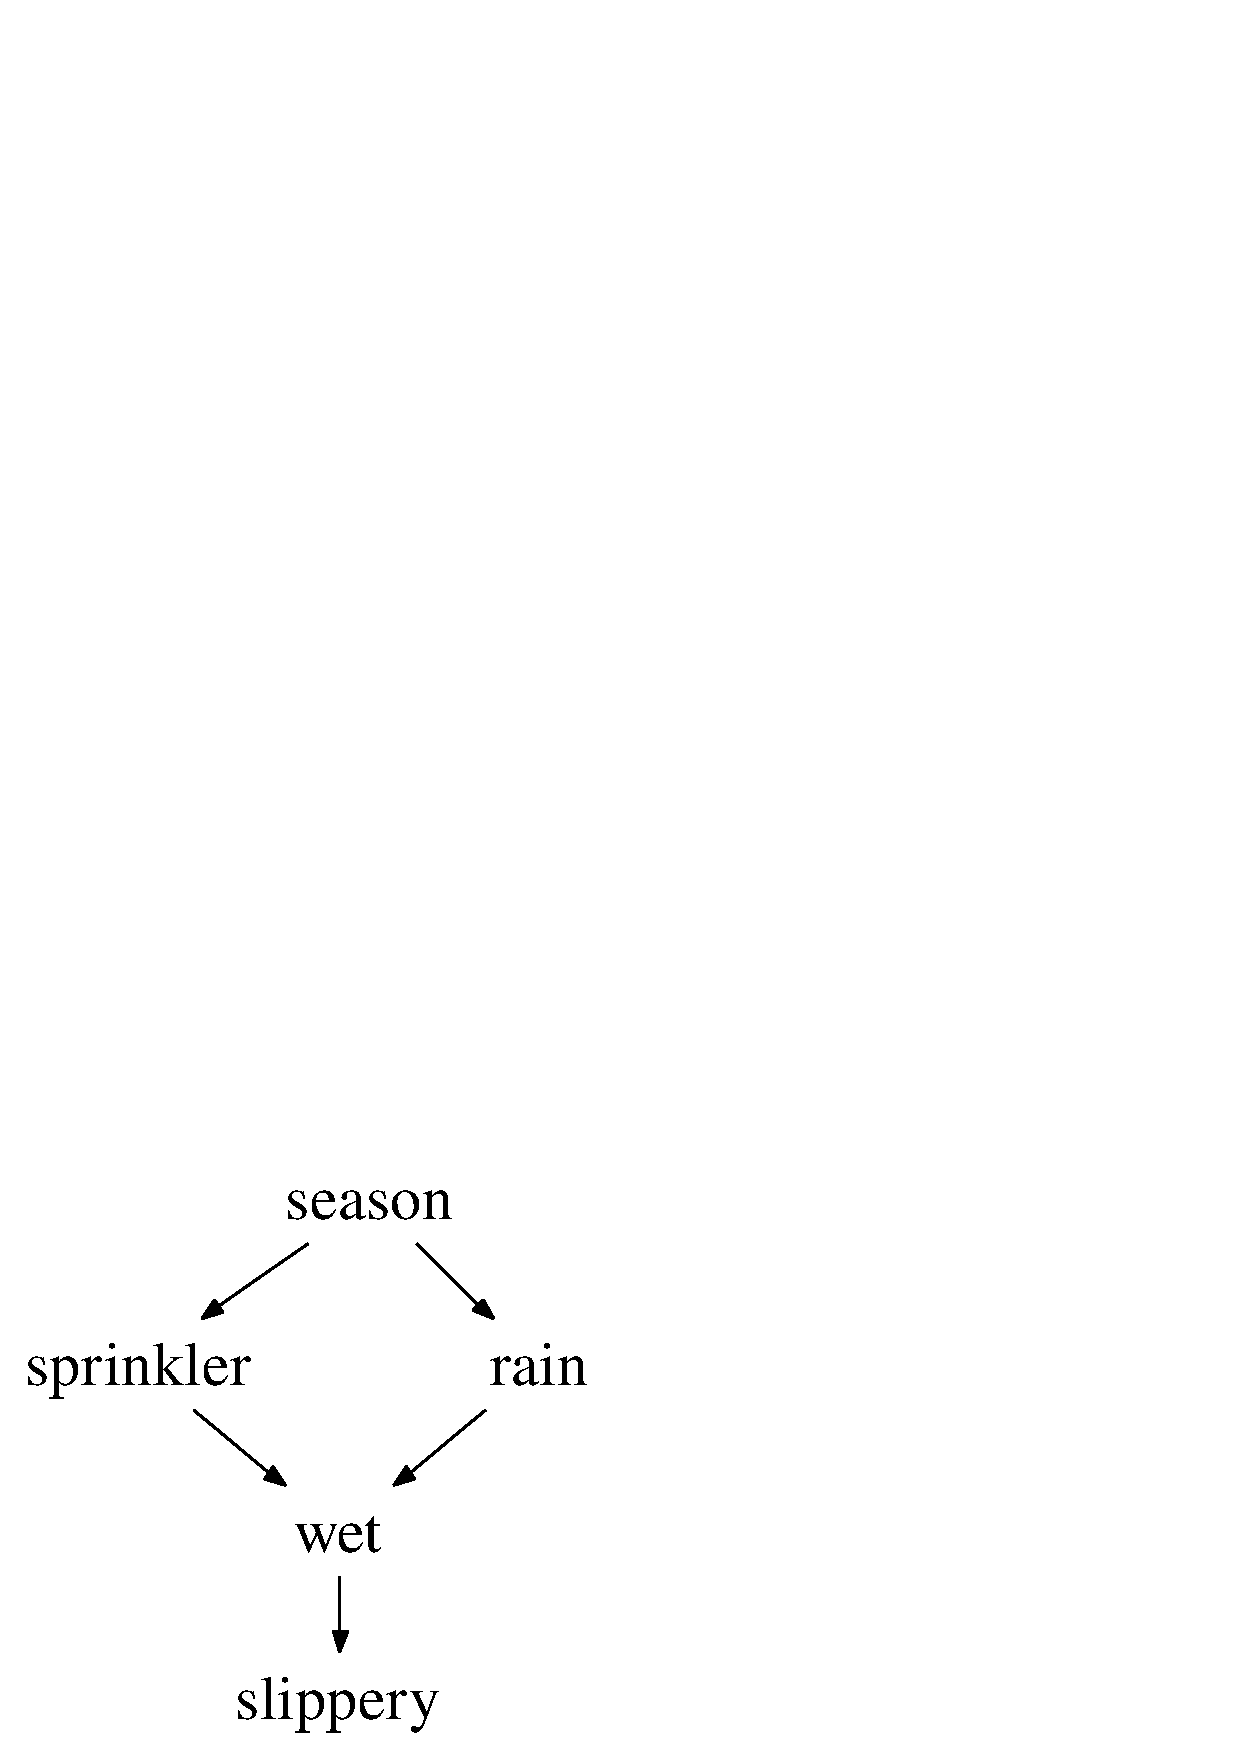
\includegraphics{sprinkler}}}
%\hspace{1cm}
\subfigure{\scalebox{0.25}{\includegraphics{sprinkler_pattern}}}
\caption{The sprinkler network (left) and its pattern (right). Sprinkler and Rain share Season as a common cause, and Wetness as a common effect. The wetness of the pavement is a direct cause of its being slippery.}%
\label{fig:sprinkler}%
\end{figure}

\subsection{Evidence Items}

An evidence item is a \textbf{conditional dependence statement} of the form 
\begin{equation} \label{eq:dependence}
\set{X} \dep \set{Y}|\set{Z}
\end{equation}

where $\set{X}$, $\set{Y}$, and $\set{Z}$ are disjoint sets of variables. Intuitively, a dependence statement can be read as ``the variables in the set $\set{\X}$ are relevant to the variables in the set $\set{\Y}$, given an assignment of values to the variables in the set $\set{\Z}$.'' 

\paragraph{Examples} 
The most common  interpretation of a dependence statement is as expressing a {\em probabilistic dependence}. Probabilistic dependencies are defined with respect to a \textbf{joint distribution} over the nodes in the graph. A joint distribution specifies a probability 

$$P(\V=\set{v})$$
for each complete assignment of values to the variables. From a joint distribution we obtain {\em marginal distributions} over any subset $\set{X}$ of variables

$$P(\set{\Y} = \set{y}) \equiv \sum_{\set{x}} P(\set{\Y} = \set{y},\set{\X} = \set{\x})$$
where $\set{\X}$ is the set of variables $\V - \set{\Y}$ other than $\set{\Y}$. 

A joint distribution also specifies {\em conditional distributions} via the definition

$$P(\set{\Y} = \set{\y}|\set{\X} = \set{\x}) \equiv \frac{P(\set{\Y} = \set{\y},\set{\X} = \set{\x})}{P(\set{\X} = \set{\x})}$$
where $\set{\X}$ and $\set{\Y}$ are disjoint, and $P(\set{\X} = \set{\x}) >0$. In what follows we assume that all joint probabilities are positive so that conditional probabilities are well defined. For a discussion of learning causal graphs with 0 joint probabilities, which may occur with deterministic causal relationships, see \cite{Luo2006a}.

The meaning of a conditional dependence statement can be defined in terms of a \textbf{probabilistic inequality} as follows:

\begin{equation} \label{eq:prob-ineq-variables} \set{X} \dep \set{Y}|\set{Z} \equiv \exists \set{\x},\set{\y},\set{\z}.P(\set{\Y} = \set{\y}|\set{\X} = \set{\x},\set{Z} = \set{z}) \neq P(\set{\Y} = \set{\y}|\set{Z} = \set{z}).
\end{equation}

For example, in the graph of Figure~\ref{fig:sprinkler}, a joint distribution may specify a probability of 0.1 that it is summer, the sprinker is on, and all other variables
are simultaneously true:

$$
P(\season = \summer, \sprinkler = \on, \rain = \true, \wet = \true, \slippery = \true) = 0.1.
$$

The joint distribution may entail the following claim: the probability that the
pavement is wet is affected by the probability that the season is summer, even
given that the sprinkler is on:

$$
P(\wet = \true|\season = \summer, \sprinkler = \on) \neq P(\wet = \true|\sprinkler = \on) 
$$
which witnesses the dependence assertion that

$$\wet \dep \season|\sprinkler.$$





\subsection{Consistency of a Causal Graph With Dependency Statements} \label{sec:bn-consistency}


For parametric models in general, a model structure is consistent with a set of evidence items if there exists an assignment of values to the model parameters that entails the observed evidence. This logic can be applied to causal graphs as follows. The parameters of a causal graph are conditional probabilities that specify, for each assignment of a value to a node, and for each assignment of values to the node's parents, the probability of the child node value, given the parent values.  The combination of (graph structure + parameters) defines a joint distribution $P$ over the nodes in the graph. Such a combination is consistent with a set of observed dependencies if the dependencies are entailed by the joint distribution $P$. A causal graph structure $\G$ by itself is then \textbf{consistent} with a set of dependence statements of the form~\ref{eq:dependence} if {\em there exists} a parameter assignment for the graph $\G$ that is consistent with the observed dependencies. Figure~\ref{fig:consistency} illustrates the logic of this definition. 


The combination of (graph structure + parameters) defines a joint distribution via the product formula: multiply together all the conditional probabilities defined by each child-parent value assignment. For instance, for the graph in Figure~\ref{fig:sprinkler}(left), the joint probability that all variables above would be defined by the product
\begin{eqnarray*}
&&P(\season = \summer, \sprinkler = \on, \rain = \true, \wet = \true, \slippery = \true)   \\
&=&P(\season = \summer) \times P(\sprinkler=\on|\season = \summer) \times P(\rain = \true|\season =  summer \\
& \times& P(\wet = \true|\sprinkler = \on, \rain = \true) \times   P(\slippery = \true|\wet = \true)
\end{eqnarray*}
where the conditional probabilities that appear in this expression are specified as parameter values for the causal graph. 


\begin{figure}[hbtp]
\centering
\resizebox{0.8\textwidth}{!}{
\includegraphics{consistency} 
}
\caption{Consistency of Causal Graph Structure with Observed Dependency Statements. A parametrized causal graph is consistent with observed dependencies if its joint distribution entails the dependencies. A causal graph structure is consistent with observed dependencies if there is a parametrization of the structure that is consistent with the dependencies.}%
\label{fig:consistency}%
\end{figure}
Causal graphs allow us to compute joint probabilities that describe the effects of interventions. For example, suppose we turn on the sprinkler given the causal structure of Figure~\ref{fig:sprinkler}. The joint distribution given this intervention can be computed by removing the edge $\season \rightarrow \sprinkler$---which represents that the value $\sprinkler$ has been determined exogenously outside the system---and using the conditional probabilities in the resulting truncated graph to compute joint probabilities. For more examples and details please see \cite{pearl00:_causal}.

\paragraph{Graph Dependencies and d-Separation}
It may appear that determining whether a graph structure $\G$ is consistent with a given set of dependencies is difficult because searching through the set of all possible parameter assignments is difficult. However, causal graph theory has developed a graph-based criterion, known as {\em d-separation}, that facilitates an efficient check whether a graph structure is consistent with given dependencies based on the links only, without reference to parameter values. For readers unfamiliar with this criterion, we provide a review in the appendix. In terms of d-separation, a causal graph structure is consistent with observed dependencies if it is an I-map of the given dependencies. This means that if any node set $ \set{X}$ is d-separated from another $ \set{Y}$ by the nodes $\set{Z}$, then the dependency statement $\set{X} \dep \set{Y}|\set{Z}$ is not in the given dependencies. 

The d-separation criterion also makes it possible to provide a graphical characterization of causal graphs that are empirically equivalent, that is, that are consistent with exactly the same set of dependency statements. Two nodes $X,Y$ are {\bf adjacent} in a graph $\G$ if $\G$ contains an edge $\X \rightarrow \Y$ or $\Y \rightarrow \X$. 
The {\bf pattern} of DAG $\G$ is
the partially directed graph that has the same adjacencies as $\G$,
and contains an arrowhead $\X \rightarrow \Y$ if and only if $\G$ contains a
triple $\X \rightarrow \Y \leftarrow \Z$ where $\X$ and $\Z$ are not adjacent. Figure~\ref{fig:sprinkler} (right) illustrates the concept. Verma and Pearl proved that two graphs $\G_1$
and $\G_2$ are consistent with the same dependency statements if and only if they lead to the same pattern
\cite[Thm. 1]{verma90:_equiv_synth_causal_model}). Thus we can use a pattern as a syntactic representation of an empirical equivalence class of graphs. This completes our description of causal graph learning as an instance of a learning problem: Evidence items are conditional dependence statements, hypotheses are patterns (equivalence classes of causal graphs), and a hypothesis is consistent with a set of dependence statements if the dependencies are entailed by applying d-separation to the graph. We next discuss the assumptions and limitations of this model (see also the predecessor paper by Schulte {\em et al.} \cite{Schulte2010}).

%new text starts here

\section{Discussion: Assumptions and Limitations}
The key assumptions are characteristic of all learning-theoretic applications, concerning the correctness and completeness of the available evidence, as well as the adequacy of the hypotheses under consideration. We discuss how our assumptions relate to previous work on learning causal graphs.


\paragraph{Approaches to Learning Causal Graphs}
There are two well established general approaches to learning a causal graph, or Bayesian network structure. {\em Constraint-based} (CB) methods employ a statistical test to detect conditional (in)dependencies given a data sample, and then compute a graph structure that fits the (in)dependencies \cite{cooper99:_comput_causat_discov,peter00:_causat}. {\em Score-based} methods search for models that maximize a model selection score~\cite{Heckerman1998}. Statistical model selection scores typically balance model fit---measured by the likelihood of the data under the model---against model complexity---often measured by the number of model parameters. For example, the AIC score subtracts the number of model parameters from the data likelihood. A key difference is that a statistical model selection score measures the fit of a model to data as a continuous quantity that comes in degrees. As the name ``constraint'' suggest, CB methods evaluate graphs in a Boolean fashion against the data: a graph either satisfies the observed (in)dependencies or not. Our paper falls in the CB paradigm, because CB methods are based on a discrete notion of consistency that allows us to apply learning-theoretic analysis. An alternative recent approach to applying learning theory to statistical problem is to develop the theory directly for probabilistic models~\cite{Kelly2010,Genin2017}, where consistency is taken to be a matter of degree. 


\paragraph{Obtaining Dependence Statements from Statistical Tests}
A dependence statement existentially quantifies over possible values of variables: it asserts that there exist specific values $\set{\x},\set{\y},\set{\z}$ such that if   the conditioning variable set $\set{Z}$ takes on the values $\set{\z}$, then the values $\set{x}$ for $\set{\X}$ do not affect the probability that $\set{\Y}$ takes on value $\set{y}$. This existentially quantified statement can be derived from basic unquantified probabilistic inequalities of the form

\begin{equation} \label{eq:basic-ineq}
P(\set{\Y} = \set{\y}|\set{\X} = \set{\x},\set{Z} = \set{z}) \neq P(\set{\Y} = \set{\y}|\set{Z} = \set{z})
\end{equation}

for fixed values $\set{\x},\set{\y},\set{\z}$. Such basic probabilistic inequalities can be ascertained  using statistical tests. In practice, a Bayesian network structure learner obtains a random sample $\d$
drawn from the data generating joint distribution over the variables $\mathbf{V}$,
and applies a suitable statistical criterion to decide if a dependency $X \protect\dep Y | \mathbf{S}$ holds \cite{peter00:_causat}, \cite[Sec.4]{bib:max-min}. Many constraint-based approaches to learning causal graphs use a statistical test as follows: given a query ``Does $X \dep Y | \mathbf{S}$ hold?'', the system answers ``yes'' if the test rejects the hypothesis $X \protect\indep Y | \mathbf{S}$, and 
``no'' otherwise. The assumption that this procedure yields correct results is called the assumption of valid statistical testing
\cite[Sect.6.2]{cooper99:_comput_causat_discov}.
Compared to this assumption, our model of learning from conditional dependencies (positive data) is  more realistic in two respects. First, the model assumes only that \emph{dependency information} is available,
but does not rely on
{\em independence} data. In fact, many statisticians hold that no independence conclusion
should be drawn when a statistical significance test fails to reject an independence hypothesis \cite{giere72:_signif_test_contr}, because there is no bound on the probability of falsely accepting an independence hypothesis after a failure to reject.\footnote{Schulte {\em et al.} \cite{Schulte2010} describe the Occam method for learning from independencies as evidence items.} Second, the dependency learning model does not assume that the dependency information is supplied by an oracle all at once, but explicitly considers learning in a setting where more information becomes available as the sample size increases. Our model still assumes that a statistically significant correlation does not disappear as the sample size increases.  The extent to  which this assumption is plausible depends on the testing strategy that extracts correlations from the given samples. The most common approach in constraint-based methods is to employ a fixed conservative significance level (e.g., $\alpha = 0.1\%$ 
\cite[Ch.5]{peter00:_causat}, \cite{campos06:_bayes}, \cite{bib:max-min}) for any sample size; with this kind of testing strategy, our assumption that the store of observed correlations grows monotonically is quite plausible. 

\paragraph{Complete Data Enumeration} This observation supports the standard assumption in learning theory that a complete infinite data stream enumerates exactly the true evidence items; in our case, the dependencies that are true in a domain. 

\paragraph{Adequacy of Hypothesis Space} In addition, the learning model model assumes that these true domain dependencies can be  represented exactly by a causal graph. In causal graph theory, this assumption is known as {\em faithfulness}. For discussions of the faithfulness assumption, see \cite[Ch.2.4]{pearl00:_causal},
\cite{xiang96:_critic_remar_singl_link_searc}, \cite[Ch.8.1]{studeny05:_probab_condit_indep_struc}).




%Dependence statements illustrate therefore the point of Section~\ref{sec:general-def} that evidence items can be higher-level aggregates of the original data: First statistical tests are applied to discover basic probabilistic inequalities for specific values, of the form~\eqref{eq:basic-ineq}. Second, these inequalities are aggregated into an existence statement that constrains only the relationships between {\em variables} of the form~\eqref{eq:prob-ineq-variables}, not between specific values. In Section~\ref{sec:context} below we consider learning from probabilistic inequalities for specific values. 

%\newtext{
%It is also possible to take as evidence items probabilistic {\em in}dependencies among variables, which are just the negations of probabilistic dependencies among variables.  Many methods for learning causal graphs are based on observed independencies rather than dependencies \cite{pearl00:_causal,peter00:_causat},\cite[Sect.6.2]{cooper99:_comput_causat_discov}.
%Schulte {\em et al.} provide a learning-theoretic analysis of such a model \cite{Schulte2010}. One reason for taking dependencies rather than independencies as learning input is motivated is that many statisticians hold that no independence conclusion
%should be drawn when a statistical significance test fails to reject an independence hypothesis \cite{giere72:_signif_test_contr},\cite{bib:kev-causal}. 
%}




As the causal graph example shows, defining the three components of a learning problem for  a realistic scenario can be a substantial task. Once this is accomplished, we can apply powerful results from general learning theory to determine optimal learning algorithms for the learning problem. We review some of these general results and apply them to causal graph structure learning in the next section. 

\section{Learning Methods and Optimal Learning}

We generically denote learners by upper-case Greek letters such as $\learnera, \learnerb$.
Intuitively, a \textbf{learner} takes as input a sequence of evidence items---called the \textbf{data sequence}, and produces as output a member of the hypothesis space. 
It is often convenient to slightly generalize this learning model: First, we allow the data sequence to contain the special non-evidence symbol $\{\#\}$ to model pauses in
data presentation. Second, we allow the learner to output $\{?\}$, where ? corresponds to the vacuous output ``no guess".  

Figure~\ref{fig:problem} illustrates these concepts. There are three evidence sequences, 
$$(2), (2,1), (2,1,3).$$ The learner maps these to a sequence of conjectures outputs $$\{2\},\{1,2\},\{1,2,3\}.$$ Each output is consistent with exactly the observed items. 


\subsection{Performance Criteria for Learning}

Learning theorists have studied a number  of performance criteria for succesful learning (often referred to as identification criteria \cite{Case.Smith:83}). In this paper we consider three: i) reliable identification of a correct hypothesis in the limit, ii) steady identification of a correct hypothesis, i.e., minimizing hypothesis changes, and iii) fast identification of a correct hypothesis, i.e., minimizing time to convergence. 

We say that a learner \textbf{identifies} a correct hypothesis on an infinite data stream if after some finite time, the learner outputs a hypothesis that is correct for the entire data stream. Identification requires induction in the sense of going beyond the data: although the learner typically has not observed all evidence items that may appear, the hypothesis it selects does concern future evidence items. A learner \textbf{reliably identifies} the correct hypothesis in a learning problem if it identifies a correct hypothesis on every possible data stream. To illustrate these concepts in the example of Figure~\ref{fig:problem}, consider the infinite data stream

$$2,1,3,\#,\#,\ldots.$$

The set of evidence items for this data stream is $\{1,2,3\}$, so the learner converges to a correct hypothesis after three evidence items have been observed. Figure~\ref{fig:learners} provides more examples of evidence and hypothesis sequences.

\begin{figure}[htbp]
\centering
\resizebox{1\textwidth}{!}{
\includegraphics{learners}
}
\caption{Examples of different learning methods. After each evidence is received, a learner outputs a hypothesis.}
\label{fig:learners}
\end{figure}


Identifiability requires only eventual convergence. We can compare the performance of different learners with respect to convergence speed by using the decision-theoretic criterion of weak dominance: A learner $\learnera$ is \textbf{faster than} a learner $\learnerb$ on a data stream if $\learnera$ converges to a hypothesis before $\learnerb$ does. A learner $\learnera$ is \textbf{uniformly faster} than $\learnerb$ if $\learnera$ is faster than $\learnerb$ on some possible data stream, and $\learnera$ is at least as fast as $\learnerb$ on every possible data stream.

Our final criterion is steadiness of convergence: minimizing the number of times that a learner changes its hypothesis before convergence. A learner $\learnera$ \textbf{changes its mind} at some nonempty finite sequence of evidence items $\langle e_{1},\ldots,e_{m},e_{m+1}\rangle$ if the output of $\learnera$ after observing evidence items $\langle e_{1},\ldots,e_{m}\rangle$ is not vacuous (i.e., is not ?) and differs from the output of $\learnera$ after observing evidence items $\langle e_{1},\ldots,e_{m},e_{m+1}\rangle$~\cite[Ch.12.2]{jain99:_system_that_learn},~\cite{putnam65:_trial_error_predic_solut_probl_mostow,bib:kev-causal}. For any possible data stream, we can count the number of mind changes that a learner undergoes on that data stream. This is a finite number assuming that the learner eventually settles on a correct hypothesis. 



We can assess the performance of a learner with respect to mind changes by using the decision-theoretic minimax criterion, which considers worst-case performance.\footnote{Schulte shows that applying admissibility to mind changes is not fruitful \cite{bib:bjps}.} Say that a learner $\learnera$ reliably identifies a correct hypothesis with at most $k$ mind changes if it is reliable and changes its hypotheses at most $k$ times on every possible data stream. In the toy problem of Figure~\ref{fig:problem}, a learner can reliably identify a correct hypothesis with at most two mind changes. This is illustrated by the Occam learner shown in Figure~\ref{fig:problem} and in the left two examples of Figure~\ref{fig:learners}. The Occam learner outputs a hypothesis that accommodates a minimum number of evidence items, if there is a unique such hypothesis. If there is not, the learner outputs ?.

A natural alternative is to express uncertainty by a set (disjunction) of hypotheses as possible outputs rather than ?. The meaning of an output is then that the true hypothesis is a member of the set. For example, a learner could output a set of languages, or a set of causal graphs. A mind change is then said to occur at $\langle e_{1},\ldots,e_{m},e_{m+1}\rangle$ if the set of hypotheses of $\learnera$ after observing evidence items $\langle e_{1},\ldots,e_{m}\rangle$ is not entailed by the output of $\learnera$ after observing evidence items $\langle e_{1},\ldots,e_{m},e_{m+1}\rangle$. (In symbols, $\learnera(\langle e_{1},\ldots,e_{m}\rangle) \not\supseteq \learnera(\langle e_{1},\ldots,e_{m},,e_{m+1}\rangle)$.) The results about problem complexity and learning optimality remain the same, so we keep with the simpler traditional ? representation in formal learning theory~\cite[Ch.12.2]{jain99:_system_that_learn}.
A global mind change bound is not quite good enough in many problems, because a learner may fail to take advantage of a lucky evidence sequence that makes it possible to learn with fewer mind changes than in the worst case. The top half of Figure~\ref{fig:learners} illustrates this possibility. After evidence item 1 is observed, it is possible to succeed with at most one further mind change: wait with ? until further evidence decides between the hypotheses $\{1,2\}$ or $\{1,3\}$. Then at most one more mind change is required if the correct hypothesis turns out to be $\{1,2,3\}$. The learner in the top right box outputs $\{1,3\}$ right away and undergoes two mind changes in case the item $2$ is observed before $3$. Since the problem requires two mind changes in the worst case (see Figure~\ref{fig:problem}), this behavior is consistent with a global mind change bound of two. We therefore refine the mind change criterion as follows \cite{Schulte2010}. Say that a learning problem can be solved with at most $k$ mind changes starting with evidence sequence $\langle e_{1},\ldots,e_{m}\rangle$ if for every data stream extending the evidence sequence, there is a learner that reliably identifies a correct hypothesis, and uses at most $k$ mind changes, where mind changes are counted starting at time $m$. That is, mind changes are counted with the output for $\langle e_{1},\ldots,e_{m}\rangle$ as the initial hypothesis. A
learner $\learnera$ is \textbf{strongly mind change optimal} if for every finite evidence sequence $\langle e_{1},\ldots,e_{m}\rangle$, the learner $\learnera$ solves the learning problem with the best possible mind change bound starting with $\langle e_{1},\ldots,e_{m}\rangle$.

\subsection{Optimal Learning}
Performance criteria can be used to select learning methods. We can picture a performance criterion as a filter that is applied to learning methods: applying multiple performance criteria is like applying successive filters to learning. The criteria we examine in the rest of the paper are as follows. 

First, filter out all methods that do not reliably identify a correct hypothesis.  Second, eliminate among the remaining ones those methods that are uniformly slower than another remaining method. Third, among these, filter out those that are not strongly mind change optimal. We refer to a method that meets these criteria simply as \textbf{optimal}. In decision-theoretic terms, the successive filters correspond to a lexicographic ordering of performance criteria: identifiability first,  convergence time second, mind change optimality third. Other combinations of performance criteria lead to different concepts of optimality; the optimality concept of this paper is the most fruitful for applications \cite{bib:bjps, bib:kev-causal}.

 The lexicographic concept is surprisingly powerful: we will show next that in many problems, including those with finite hypothesis spaces, there is only one optimal method. This optimal method guides us towards interesting and plausible inductive inferences in many domains. Determining the hypotheses selected by the optimal method is an investigation that leads to substantive insights into the methodological structure of a learning problem.  We outline a general result that assists a theorist in determining the conjecture of the optimal method. Then we show how to apply this to causal graph search.


%\subsection{Global Underdetermination}
%Some issues with the performance criteria arise when different hypotheses are \textbf{empirically equivalent}, meaning that they are consistent with exactly the same evidence items. This occurs in many practical hypothesis spaces, because hypotheses are described using a hypothesis language, and just like natural language, a hypothesis language typically allows us to express the same content in different ways. For example one set of conservation laws is empirically equivalent to another if they both span the same linear subspace \cite{schulte}. We discuss empirical equivalence in causal graphs in Section~\ref{sec:graph-occam} below. In philosophical discussions of inductive inference, this phenomenon is often described as global underdetermination. In statistical terminology, it is referred to as the identifiability problem, where even an infinitely large sample does not entail a uniquely correct model and/or parameter values for the model. For reliable convergence to a correct hypothesis, global underdetermination raises the problem of defining which hypothesis is the correct one for a data stream when there are empirically equivalent alternatives. It is even possible for a method to cycle among equally correct alternatives forever without settling on one \cite{behavioural}, which is arguably an alternative concept of convergence to a correct hypothesis. Similarly, for mind changes, we may not want to count switching from one empirically equivalent hypothesis to another as a mind change. A simple approach to global underdetermination is to have learners output an equivalence class of hypotheses. In effect, this changes the hypothesis space to such that a hypothesis in the new space is an equivalence class of hypotheses in the original space. A benefit of this approach is that in many problems, determining which hypotheses are empirically equivalent is a problem of independent interest. As we show in the causal learning example, an equivalence class of original hypotheses can be often be described compactly. In the following we assume that learners output equivalence classes of hypotheses.

\section{Optimal Learning and Inductive Simplicity}

Our goals in this section are to prove the uniqueness of an optimal learner and to characterize optimal inferences in terms of the structure of the learning problem. This structure can be described in terms of a topological ranking of hypotheses in a given hypothesis space \cite{luo06:_mind_chang_effic_learn}. 

\begin{definition}
Let $\hypotheses$ be a hypothesis space and $\hypothesis$ be
a hypothesis in $\hypotheses$. We write $\hypothesis \subset \hypothesis'$ to denote that the evidence items consistent with hypothesis $\hypothesis$ are a proper subset of those consistent with $\hypothesis'$. An \textbf{inclusion chain} of length $k$ starting with $\hypothesis$ is a sequence of the form 
\[ 
\hypothesis \subset \hypothesis_1\subset
\dots\subset \hypothesis_i\subset \dots\subset \hypothesis_k
\]
where each hypothesis in the chain is contained in the hypothesis space $\hypotheses$. The \textbf{inclusion depth}
of $\hypothesis$ is the maximum length of an inclusion chain starting with $\hypothesis$.
\end{definition}

Kevin Kelly has developed the view that inclusion depth, or closely related concepts, can be viewed as a simplicity ranking of hypotheses~\cite{kelly04:_justif_truth_findin_effic}. Accordingly, we define the \textbf{inductive simplicity rank} of a hypothesis $\hypothesis$ in a learning problem as the inclusion depth of $\hypothesis$. Thus defined, simplicity increases with inclusion depth. Occam's razor directs us to adopt a maximally simple hypothesis that is consistent with the evidence. For a learning problem, this leads to the following definition of the \textbf{Occam learner}

$$
\occam(\langle e_{1},\ldots,e_{m}\rangle)=
\begin{cases}
? & \text{if there is no uniquely simplest hypothesis consistent with  }\langle e_{1},\ldots,e_{m}\rangle\\
\hypothesis & \text{if $\hypothesis$ is the uniquely simplest hypothesis consistent with  }\langle e_{1},\ldots,e_{m}\rangle
\end{cases}
$$

\noindent where $\occam(\langle e_{1},\ldots,e_{m}\rangle)$ is the output of the Occam learner after receiving the evidence sequence $\langle e_{1},\ldots,e_{m}\rangle$. This definition assumes that there are no empirically equivalent hypotheses; otherwise it should be modified so that the Occam learner outputs the maximally simple equivalence class if there is one. 

The next proposition shows a strong connection between inductive simplicity and required mind changes: The worst case number of mind changes required is exactly the maximum of the inductive simplicity ranks in the hypothesis space. 

\begin{proposition}[Luo and Schulte 2006] \label{prop:mc-char}
For any learning problem with a finite hypothesis space, there is a learner that reliably identifies a correct hypothesis with at most $k$ mind changes $\iff$ the maximum inductive simplicity rank of any hypothesis is $k$.
\end{proposition}

\begin{proof}
$(\Leftarrow)$ Suppose that the maximum inductive simplicity rank of any hypothesis is $k$. Consider a mind change by the Occam learner $\occam$ on a sequence of evidence items $\langle e_{1},\ldots,e_{m},e_{m+1}\rangle$. Let $\hypothesis$ be the output of $\occam$ on the previous sequence  $\langle e_{1},\ldots,e_{m}\rangle$. Since a mind change occurred at stage $m+1$, the hypothesis $\hypothesis$ is not vacuous. By the definition of the Occam learner, $\hypothesis$ is therefore the uniquely most simple consistent with the evidence $\langle e_{1},\ldots,e_{m}\rangle$. Thus any other hypothesis consistent with the further evidence $\langle e_{1},\ldots,e_{m},e_{m+1}\rangle$ must have lower simplicity rank than $\hypothesis$. Therefore any time that the Occam learner changes its mind, the maximum simplicity rank of the remaining hypotheses decreases by at least 1. Since the maximum rank over all is $k$, there can be at most $k$ mind changes by the Occam learner.

$(\Rightarrow)$ Let $\learnera$ be an arbitrary learner. Suppose that there exists an inclusion chain 
\[ 
\hypothesis \subset \hypothesis_1\subset
\dots\subset \hypothesis_i\subset \dots\subset \hypothesis_k.
\]
There is a possible data stream that enumerates all and only evidence items that are consistent with $\hypothesis$. On this data stream, the learner $\learnera$ must output $\hypothesis$ at some finite stage $m$ to converge to the correct hypothesis. At this point, there is a data stream that extends the finite evidence sequence and enumerates all and only evidence items that are consistent with $\hypothesis_{1}$. Again the learner $\learnera$ must output $\hypothesis_{1}$ at some finite stage $m_{1}$ to converge to the correct hypothesis. This leads to at least one mind change by the learner. Repeating this argument, we can extend the data streams after the mind change occurs consistent with hypotheses $\hypothesis_{2}, \ldots,\hypothesis_{i},\ldots,\hypothesis_k$, in such a way that a mind change occurs for each hypothesis in the chain. The result is a data stream on which the learner $\learnera$ requires at  least $k$ mind changes. Since $\learnera$ is an arbitrary learner, the construction shows that in the worst case, every learner requires at least $k$ mind changes.
\end{proof}

%A formal proof is provided by \cite{wei-mc}. 
This result can be extended to infinite hypothesis spaces using transfinite mind change bounds and a topological generalization of the concept of simplicity rank. The concept of inductive simplicity developed applies therefore in a wide class of problems. The main restriction is that learning with a mind change bound requires that some hypothesis be conclusively verifiable, in the sense that there is some evidence that is consistent only with that hypothesis. Kelly \cite{Kelly2010} presents a generalization of mind change optimality that relaxes this assumption. 

Proposition~\ref{prop:mc-char} characterizes the inductive complexity of an entire learning problem. The next proposition concerns the properties of optimal learners. The main result is that the Occam learner is the {\em only} learner that achieves reliable, steady, and fast convergence.

\begin{proposition}
\label{prop:occam}
For a finite hypothesis space, the Occam learner is the only learner that reliably identifies a correct hypothesis, is convergence-time efficient, and strongly mind change optimal.
\end{proposition}

\begin{proof-outline}
Any reliable learner is strongly mind change optimal if and only if whenever it produces a nonvacuous hypothesis, the hypothesis is the uniquely simplest consistent with the evidence. For otherwise the learner may incur one more mind change than necessary given the evidence, as illustrated in the top right box of Figure~\ref{fig:learners}. What distinguishes the Occam learner from other strongly mind change optimal learners is that the Occam learner does not wait: it immediately conjectures the  uniquely simplest hypothesis as soon as there is one, whereas other strongly mind change optimal may output ? instead. It is easy to see that the Occam learner is uniformly faster than all such learners: Since the output ? is not correct for any data stream, whenever a non-Occam learner outputs ? on an evidence sequence $\langle e_{1},\ldots,e_{m}\rangle$ , its convergence time is later than stage $m$. The Occam learner by contrast converges to the uniquely simplest hypothesis $\hypothesis$ by time $m$ on every data stream extending the evidence  $\langle e_{1},\ldots,e_{m}\rangle$ for which $\hypothesis$ is correct. Therefore the Occam learner possibly converges sooner than the non-Occam learner, and never slower. 
\end{proof-outline}

Luo and Schulte~\cite{luo06:_mind_chang_effic_learn} provide a formal proof that includes the general case of infinite hypothesis spaces. Without the requirement of convergence-time efficiency, the conjectures of a strongly mind-change optimal learner are no longer uniquely determined, because the learner can always wait for more evidence to make a conjecture without selecting a hypothesis. This is a reasonable inductive strategy in many cases. However, as the argument above showed, it remains the case that when the learner does eventually change its mind, it must be to adopt a unique maximally simple hypothesis. Implementing the Occam learner requires determining the simplicity rank of a hypothesis. In the next section we determine the simplicity rank of causal graphs. 

\section{Inductive Simplicity for Learning Causal Graphs}
\label{sec:graph-simplicity}

In this section we characterize the inductive simplicity rank of a causal graph and the Occam learner for causal graphs. 

A fundamental result in causal graph theory characterizes the inclusion relation between two causal graphs $\G_{1} \subset \G_{2}$, meaning that $\G_{2}$ is consistent with all dependency statements that are consistent with $\G_{1}$. The Meek-Chickering theorem shows that the inclusion holds just in case $\G_{2}$ can be transformed into $\G_{1}$ by a sequence of two types of transformations: (i) deleting edges, and (ii) reversing a covered arc \cite{meek97:_graph_modeln},\cite[Thm.4]{Chickering2003}. For definitions, please see \cite{Schulte2010}. 

\begin{figure}[htbp]
\centering
\resizebox{0.6\textwidth}{!}{
\includegraphics{bn-inclusion}
}
\caption{Left: An inclusion chain among causal graph patterns. The dependencies of the bottom pattern are included in those for the middle pattern which are included in those for the top patterns. Right: Representative dependency statements for each pattern. In figures we use the notation $Dep(A,B|C)$ for $\A\dep |C$.}%
\label{fig:bn-inclusion}%
\end{figure}


The Meek-Chickering theorem is the basis for the following characterization of inductive simplicity for causal graphs. 

\begin{proposition}
The inductive simplicity rank of a causal graph or pattern containing edges $\set{E}$ is $|\V|-|\set{E}|$, the number of edges that are {\em not} included in the graph.
\end{proposition}
 
 The formal proof can be found in \cite{Schulte2010}. So the simplest graph is the empty one, and the most complex graph is the complete one that contains all possible adjacencies. It is not surprising that the inductive complexity of a graph increases with the number of edges in the graph. The surprising aspect of the proposition is that the number of edges is all that matters: the direction of the adjacencies does not affect the simplicity rank. 

The Occam learner for causal graph learning is therefore as folllows. Let $\D$ be a list of observed dependencies.

$$
\occam(\D)=
\begin{cases}
? & \text{if there is no uniquely simplest pattern consistent with the dependencies }\D\\
\G & \text{if $\G$ is the uniquely simplest pattern consistent with  }\D.
\end{cases}
$$

Figure~\ref{fig:occam-learn} illustrates some of the hypotheses of the Occam learner. Schulte {\em et al.}~\cite{Schulte2010} provide a more elaborate example for a graph with four nodes. 

\begin{figure}[htbp]
\centering
\resizebox{0.9\textwidth}{!}{
\includegraphics{occam-learn}
}
\caption{The hypotheses of the Occam learner on a sequence of three observed dependency statements.}%
\label{fig:occam-learn}%
\end{figure}

As the number of variables increases, it becomes challenging to determine whether there is a  uniquely optimal causal graph for a given list of observed correlations. Schulte {\em et al.} \cite[Th.23]{Schulte2010} show that computing the outputs of an Occam learner is NP-hard. Therefore we can conclude that there is no algorithm that implements the Occam learner exactly in reasonable (polynomial) computation time. Researchers in causal graph learning have developed a number of heuristic search algorithms that can be seen as approximating the Occam learner~\cite{Schulte2010a}.

So far we have considered the problem of learning causal relationships among {\em variables}. However, some causal relationships involve specific values of variables. In the next section, we examine causal learning with Occam's razor for variable values. 


\section{The Occam Learner for Causal Context-Sensitive Causal Relationships} \label{sec:context}

We provide a motivation for our approach and overview of our results, then go into the technical details. 

\subsection{Context-Sensitive Dependencies: Overview and Motivation}
For discrete variables, it is common that a causal relationship holds not in general, but only conditional on the values of some variables \cite{Boutilier1996, Geiger1996, friedman98:_learn_bayes}. These values establish a {\em context} that may reveal additional causal relationships. For a simple example, there may be a causal relationship between the intelligence of a student and their grade in a course. But this relationship holds only 
for students actually registered in the course, that is, conditional on Registration being true.
Geiger and Heckerman discuss the following example~\cite{Geiger1996}. Figure~\ref{fig:geiger-bn} shows a Bayesian network structure for this example.

\begin{quote}
A guard of a secured building expects three types of persons to approach the building's entrance: workers in the building, approved visitors, and spies. As a person approaches the building, the guard can note its gender and whether or not the person wears a badge. Spies are mostly men. Spies always wear badges in an attempt to fool the guard. Visitors don’t wear badges because they don’t have one. Female workers tend to wear badges more often than do male workers. The task of the guard is to identify the type of person approaching the building.
\end{quote}


 
\begin{figure}[htbp]
\centering
\resizebox{0.6\textwidth}{!}{
\includegraphics{geiger-bn.png}
}
\caption{A Bayesian network for Geiger and Heckerman's security guard example. The type of a person predicts its gender (spies are mostly men). Conditional on $\it{Type = Worker}$, $\it{Gender}$ predicts the wearing of a badge. However, conditional on $\it{Type = Visitor}$ or on $\it{Type = Spy}$, $\it{Gender}$ and $\it{Badge}$ are independent. However, the graph structure is consistent with every dependency assertion, and fails to represent the two context-sensitive independencies.}%
\label{fig:geiger-bn}%
\end{figure}



%Context-sensitive (in)dependencies \cite{Boutilier1996} are also called asymetric independencies \cite{geiger}. 
Therefore for workers, gender is causally related to wearing a badge, but for spies and visitors, it is not. As Figure~\ref{fig:geiger-bn} illustrates, a single graph structure cannot represent this pattern explicitly, only implicitly through setting appropriate conditional probability parameters. An explicit context-sensitive representation of conditional probabilities conveys more information to the user, improves statistical efficiency, and facilitates faster inference to answer probabilistic queries~\cite{Boutilier1996,friedman98:_learn_bayes,Boutilier1999}.  % using d-separation. 
Combining learning causal graphs and context-sensitive independencies suggests a two-part approach: first, employ an Occam learner to find a maximally simple graph with a minimum number of edges, then another Occam method to find a maximally simple representation of context-sensitive (in)dependencies between a child node and its parents.

One approach to representing context-sensitive (in)dependencies is to employ different causal graphs for different contexts, as in multinets or similarity networks~\cite{Geiger1996}. Another is to employ a structured representation of the conditional probability parameters \cite{lauritzen88:_local,Boutilier1996,friedman98:_learn_bayes,Provost2003}. 
 %Perhaps the most common approach has been to augment a causal graph with probability estimation trees for representing context-sensitive (in)dependencies between some parent nodes and a child node, given specific settings of other parent nodes. 
{\em Probability estimation diagrams} \cite{Boutilier1999} are an intuitive formalism that provides a compact structured representation of conditional probabilities (see Figure~\ref{fig:pet} below for an example).  In this section we examine {\em the mind-change optimal Occam learner for identifying a probability estimation diagram.}

Our main result is that the inclusion depth complexity of a PED is given by the number of its terminal nodes (with no children). The number of terminal nodes is equivalent to the number of parameters required to specify a joint distribution. Inductive simplicity as defined in terms of inclusion chain therefore agrees with standard statistical model selection criteria, such as BIC and AIC, in measuring the complexity of a PED by the number of its parameters, but offers a novel justification for minimizing the number of parameters: selecting the simplest PED consistent with the observed dependencies minimizes the number of worst-case mind changes a causal dependency learner may have to undergo. Statistical model selection criteria do not usually take into account the number of edges in a causal graph.\footnote{An exception is the minimum message length criterion, which explicitly includes both the number of edges and the number of parameters in an additive overall complexity measures \cite{Dowe2011}.}
  However, because the number of parameters increases with the number of edges, for many graphs ranking by the number of parameters leads to very similar to results as our two-part scheme. We next give the formal definitions to develop our technical results. 


%~\cite{friedman98:_learn_bayes}. 



\subsection{Probability Estimation Diagrams} 
 In what follows we consider a fixed graph structure $\G$ and a node $\childvar$ in the graph. The parents of $\childvar$ are denoted $\parentvar_{1},\ldots,\parentvar_{\numparents}$. 
In causal terminology, the child node $\childvar$ represents a dependent or outcome variable, 
and the parent nodes $\parentvar_{i}$ represent independent or treatment variables. 
 An assignment of $\numparents$ values to each independent variable is denoted by boldface notation such as $\parentvals,\parentvals'$. The parameters of a causal graph specify conditional probabilities of the form
 $$P(\childvar = \childvarvalue|\parentvars = \parentvals).$$ Often the required conditional probabilities are specified simply by enumerating them. The result is a flat table of conditional probabilities.  A tabular representation fails to capture additional structure in the conditional distribution of the child variable given parent variable values; thus it fails to represent context-sensitive independencies.  A \textbf{probability estimation diagram} is a DAG $\tree$ whose nonterminal nodes are labelled with the parents of $\childvar$. Each terminal node (with no children) is labelled with a probability distribution over the possible values of $\childvar$.  An edge from a node labelled $\parentvar$ to a child is labelled with a possible value from the domain of $\parentvar$. The edges originating from a node labelled $\parentvar$ partition the domain of $\parentvar$, meaning that every possible value is assigned to one and only one edge. This entails that for any complete assignment of parent values, following the appropriate edges in the diagram leads to a unique terminal, which we denote as $\leaf_{\tree}(\parentvals)$. Figure~\ref{fig:pet} illustrates two probability estimation diagrams for the security guard problem. 
 
 \begin{figure}[htbp]
\centering
\resizebox{0.9\textwidth}{!}{
\includegraphics{pet}
}
\caption{Two equivalent probability estimation diagrams for the security guard graph of Figure~\ref{fig:geiger-bn}, for the child node $\it{Badge}$, and the parent nodes $\it{Type}$ and $\it{Gender}$. We define $p = P(\it{Badge} = \true)$. Both diagrams entail the same conditional dependencies and independencies.} %
\label{fig:pet}%
\end{figure}

 
Given a probability estimation diagram, {\em it is easy to translate paths in the diagram into probabilistic clauses:} logical rules with probabilities attached. For instance, one of the paths  in the left diagram of Figure~\ref{fig:pet} corresponds to the probabilistic clause

$$\it{Badge} = \true \leftarrow \it{Type = Worker}, \it{Gender = Woman}; p = 0.7.$$

Such clauses provide a way to combine the formalism of first-order logic with probabilistic reasoning~\cite{Ngo1997}. Khosravi {\em et al.} show that learning probability estimation trees (a special type of PEDs) to augment causal graph structures is a scalable way to discover probabilistic clauses that provide accurate predictions \cite{Khosravi2012a}.

  
\subsection{The Diagram Learning Problem}
 
The learning problem is to identify a probability estimation diagram structure that is sufficiently complex to represent the true conditional probability distribution of the child variable conditional on the parent variables. The evidence items for this learning problem are conditional inequalities of the form 
$$P(\childvar|\parentvars = \parentvals) \neq P(\childvar|\parentvars = \parentvals')$$
where $\parentvars$ denotes the parent variables and $\parentvals$ is an assignment of values to the parents. 
Thus an evidence item asserts that the distribution of the child variable, conditional on one assignment of values to the parent variables, differs from the distribution conditional on another assignment of values to the parent variables.  


%$$P(\childvar|\parentvars = \parentvals) \neq P(\childvar|\parentvars = \parentvals')$$
%where $\parentvars$ denotes a subset of parent variables and $\parentvals$ is an assignment of values to the subset. The parent set $\parentvars$ may contain all parents. 
%Thus an evidence item asserts that the distribution of the child variable, conditional on one assignment of values to a subset of the parent variables, differs from the distribution conditional on another assignment of values to the same parent variables.  
%


To complete the definition of the learning problem, we need to specify the set of evidence items are consistent with a diagram. 
%Say that a complete assignment of values $\parentvars = \parentvals$ to all parent variables extends a partial assignment $\partialparents = \partialparentvals$ if the two assigments agree on the parent subset $\partialparents$.
A diagram $\tree$ entails a conditional {\em equality} constraint 
$$P(\childvar|\parentvars = \parentvals) = P(\childvar|\parentvars = \parentvals')$$ if $\leaf_{\tree}(\parentvals) = \leaf_{\tree}(\parentvals')$. A diagram is \textbf{consistent with}
a conditional {\em in}equality constraint $P(\childvar|\parentvars = \parentvals) \neq P(\childvar|\parentvars = \parentvals')$  if the diagram does not entail its negation. Note that whether a diagram is consistent with an (in)equality constraint depends only on the qualitative graph structure of the diagram, not on the quantitative probability estimates in its terminals. In sum, the components of the learning problem in this section are as follows.

\begin{description}
\item[Hypothesis Space] The set of probability estimation diagram structures for a child variable $\childvar$ with parent variables $\parentvars$.
\item[Evidence Items] Conditional distribution inequalities of the form $$P(\childvar|\parentvars = \parentvals) \neq P(\childvar|\parentvars = \parentvals').$$
\item[Consistency Relation] A diagram structure is consistent with an inequality constraint $P(\childvar|\parentvars = \parentvals) \neq P(\childvar|\parentvars = \parentvals')$ if the assignments $\parentvals,\parentvals'$ are mapped to different terminals.
\end{description}

The Occam learner for this problem selects the inductively simplest diagram. In the next section we characterize the inductive simplicity rank of a probability estimation diagram.

\section{The Inductive Simplicity of a Probability Estimation Diagram} 

%We follow the same methodology as with determining the inclusion depth of a causal graph.
% The first step is to characterize the semantic inclusion relation $\hypothesis_{1} \subset \hypothesis_{2}$ between hypotheses in terms of a structural relationship between the syntactic structures that represent the hypotheses.
Different diagram structures may be empirically equivalent in the sense of being consistent with exactly the same probabilistic inequalities. An equivalence class can be characterized by a partition of parent value assignments. More precisely,
%
%It is helpful to map a diagram into a different representation of inequality constraints that is less compact but mathematically simpler. 
the terminals of a diagram induce a partition of the parent value assignments into equivalence classes, where two assignments are equivalent if they are mapped to the same terminal node:

\begin{equation} \label{eq:tree-part}
\parentvals \equiv \parentvals' \iff \leaf_{\tree}(\parentvals) = \leaf_{\tree}(\parentvals'). 
\end{equation}


 
In general, if Equation~\eqref{eq:tree-part}  holds for an equivalence partition $\partition$ and a diagram $\tree$, we say that the partition \textbf{corresponds} to the diagram. It is easy to see that two diagram structures are consistent with exactly the same probabilistic inequalities just in case they corresond to the same partition. Table~\ref{table:ped-partition} shows the partition that corresponds to the diagrams for the security guard problem.
Note that \emph{the number of terminals in a diagram equals the size of any partition that corresponds to it.} Therefore equivalent diagrams have the same number of terminals, even if their internal structure is different. 

\begin{table}[tbp] \centering
\resizebox{1\textwidth}{!}{
\begin{tabular}{l|l|l|l}
Cell 1 & Cell 2 & Cell 3 & Cell 4 \\
\hline
Visitor=T, Gender=Man & Spy=T, Gender=Man & Worker=T, Gender=Man & Worker=T, Gender=Woman \\
Visitor=T, Gender=Woman & Spy=T, Gender=Woman \\
\end{tabular}
}
\caption{Each of the two diagrams in Figure~\ref{fig:pet} corresponds to the same 4-cell partition of parent assigments, shown in the table.}%
\label{table:ped-partition}
\end{table}


%\begin{figure}[htbp]
%\centering
%\resizebox{1\textwidth}{!}{
%\includegraphics{ped-partition}
%}
%\caption{The partition of parent assigments corresponding to each of the diagrams in Figure~\ref{fig:pet}.}%
%\label{fig:ped-partition}%
%\end{figure}

It is easy to see that for every partition, there is a corresponding diagram: We can build a tree structure whose branches corresond to the possible assignment of parent values. If two assignments are equivalent, the corresponding branches end in the same terminal node. We thus have the following lemma.
% 
%The next lemma says that not only is there a partition of complete assignments for every diagram structure, but for every possible partition there is a corresponding diagram structure. This result depends on allowing edges to be labelled with more than one possible value. If an edge may only be labelled with a single possible value, the equivalence between partitions and diagram structures no longer holds, because every split on the values of a parent variable partitions all these values. 

 

\begin{lemma} \label{lemma:refine}
Consider the space of complete parent value assignments $\parentvars= \parentvals$ for a child node $\childvar$. 

\begin{enumerate}
\item For every diagram structure $\tree$, there is a corresponding partition of the parent value assignments.
\item For every such partition $\partition$, there is a corresponding diagram structure.
\end{enumerate}
\end{lemma}


%Causal graphs are often learned with a topological variable ordering, which means that for each parent appears before its children in the ordering \cite{Pearl, Koller}. We can extend this concept to trees: A tree satisfies a total ordering of the parent variables if for any nonleaf node in the tree, its predecessor appears before the node in the ordering. 
%For trees based on the same parent ordering, the refinement ordering can be characterized in terms of structure transformation in analogy with Theorem~\ref{thm:meek}. The operation of \textbf{edge splitting} introduces more edges by partitioning the possible values of a node into more subsets, and constructing a subtree for each of the new subsets. The operation of \textbf{leaf expansion} replaces a leaf node by a node labelled with a parent variable $\parentvar$ whose only successor is a single leaf node. That is, all values in the domain of $\parentvar$ map to a singe leaf.
%
%\begin{lemma} \label{lemma:refine} Let $\tree$ and $\tree'$ be two probability estimation trees for the same child variable that satisfy the same parent variable ordering. Then $\tree \leq \tree' \iff$ the tree structure $\tree$ can be transformed into the tree structure $\tree'$ by repeating the following operations: (1) edge splitting, and (2) leaf expansion. 
%\end{lemma}
%
%If two trees do not satisfy the same variable ordering, we can first transform them into two trees that do, then apply Lemma~\ref{lemma:refine} to compare the transformed trees. 
%
%Step 1: refinement.
%Step 2: transform by a) reordering. b) splitting edges. c) expanding node.

%Using a uniform ordering without making the tree more complex is possible because we allowed edges to be labelled with more than one possible value. If an edge may only be labelled with a single possible value, Proposition~\ref{prop:tree-inclusion} no longer holds. 


A diagram semantically includes another if it is consistent with more inequality constraints. Therefore diagram $\tree'$ includes $\tree$ if and only if the partition of $\tree'$ refines the partition of $\tree$; we denote this relationship by $\tree \isincluded \tree'$. 
The benefit of the partition representation is that inclusion depth in partition space is simply characterized by the size of the partition. Consider partitions of a finite set $S$ elements. So the coarsest partition has size 1, and the maximally refined partition has size $|S|$. A refinement chain starting with partition $\equiv$ is a sequence $$\equiv \isincluded \equiv_{1} \isincluded \equiv_{i} \cdots \equiv_{k},$$ where each element in the chain refines its predecessor but not vice versa. The \textbf{refinement depth} of partition $\equiv$ is the length $k$  of a refinement chain starting with partition $\equiv$. The starting partition $\equiv$ is not included in the length count.  The next proposition asserts that the refinement depth of a partition is simply the size $|S|$ of the most refined partition, minus the size of the partition. The basic reason for this is that to form a maximally long refinement chain, each partition in the chain should split exactly one cell of its predecessor into exactly two cells. Thus each partition in the chain contains exactly one more cell than its predecessor. Any other way to construct a refined partition is equivalent to merging two-way splits and therefore shortens the chain unnecessarily.

\begin{proposition}\label{char:refine-depth}
The refinement depth of a partition $\partition$ on a finite set with $N$ elements is $N-|\partition|$, where $|\partition|$ is the size of the partition.  
\end{proposition}
The proposition follows from the classical result~\cite{Lucas1990} that the rank of a partition over a finite set is $N-|\partition|$. To make the paper self-contained, we provide a direct proof in the appendix using our notation.
By the correspondence Lemma~\ref{lemma:refine}, the inclusion depth of a diagram is the refinement depth of its corresponding partition. By Proposition~\ref{char:refine-depth}, the refinement depth is the size of the partition, which equals the number of terminals in the diagram. Therefore the inclusion depth of a diagram equals the number of terminals in the diagram. We summarize our results in the following corollary.

\begin{corollary}
The inclusion depth of a diagram is the number of its terminals. Therefore
the Occam learner outputs a diagram with the minimum number of terminals, if all such diagram structures are equivalent (i.e., they are consistent with exactly the same probabilistic inequalities). Otherwise it outputs ?.
\end{corollary}

Figure~\ref{fig:occam-diagram} provides an example of the Occam learner. We leave for future work the analysis of the computational complexity of implementing the Occam learner.
%
%For a given input evidence sequence of inequality statements, a maximally simple diagram with a minimum number of terminals can be found using the Algorithm specified in the proof of Lemma~\ref{lemma:refine}. This algorithm requires runtime that is only linear in the number of parent variable assignments that appear in the data sequence. The algorithm  does not determine whether all minimum-parameter diagrams are equivalent. We leave for future work the analysis of the computational complexity of the  uniqueness problem.  

\begin{figure}[htbp]
\centering
\resizebox{1\textwidth}{!}{
\includegraphics{occam-diagram}
}
\caption{To illustrate the Occam learner for the security guard problem. We have used obvious abbreviations for variable values. The conditional probabilities are all of the form $P(\mathit{Badge} = \true|\cdot)$, abbreviated as $P(\true|\cdot)$. }%
\label{fig:occam-diagram}%
\end{figure}



\section{Conclusion}
An application of Occam’s razor to inductive inference directs us to choose the
simplest hypothesis consistent with the evidence. The principle is plausible but
vague to the extent that the concept of simplicity is undefined. Learning theorists
have developed a precise definition of inductive simplicity based on the topology
of the space of alternative hypotheses, which leads to a learning-theoretic version
of Occam's razor. The learning-theory razor can be justified in terms of learning performance:
it is the only learning method that guarantees reliable, steady, and fast convergence
to a correct hypothesis. As a case study, we applied Occam's inductive
razor to learning causal relationships from observed correlations, an important
and challenging practical problem. The Occam learner selects the causal graph
that represents the observed dependencies among variables with a minimum
number of edges. For context-sensitive dependencies, that may hold only in
a given context, the Occam learner augments the causal graph with probability
estimation diagrams that suffice to explain the observed correlations, with
a minimum number of free parameters. Probability estimation diagrams are
easily converted to probabilistic logical rules, so causal learning can be used to
discover logical rules that represent statistical patterns in the data.

The learning-theoretic version of Occam’s razor has a clear justification in
terms of learning performance guarantees. In many learning problems, including
causal modelling, it leads to plausible inferences and to substantive insights into
the methodological structure of the problem.

\section*{Acknowledgements}
% \paragraph{\textbf{Acknowledgements}}
% \label{sec:acknowledgements}
%Kevin T. Kelly suggested considering Bayes net learning based on conditional dependencies rather than independencies. %Tetrad group. Kevin is properly cited.
This research was supported by an NSERC discovery grant to the author.
Preliminary results were presented at the Center for Formal Epistemology at
Carnegie Mellon University. The author is grateful to the audience at the Center
for helpful comments.

\section*{Proof of Proposition~\ref{char:refine-depth}}
%\begin{lemma} \label{lemma:refine}
%Consider the space of complete parent value assignments $\parentvars= \parentvals$ for a child node $\childvar$. 
%
%\begin{enumerate}
%\item For every diagram structure $\tree$, there is a corresponding partition of the parent value assignments.
%\item For every such partition $\partition$, there is a corresponding diagram structure.
%\end{enumerate}
%\end{lemma}
%\begin{proof}
%Part 1: Since each parent value assignment is mapped to a unique leaf value, the set of assignments that reach a leaf form an equivalence class (see .
%
%Part 2: Consider a partition $\partition$. Choose an arbitrary ordering $\parentvar_{1}, \parentvar_{2},\ldots,\parentvar_{\numparents}$ of the parent variables. The diagram is constructed as follows. The root node is labelled with $\parentvar_{1}$. Consider two values $\parentval,\parentval'$ in the domain of $\parentvar_{1}$,  and any two complete assignments $\parentvals, \parentvals'$ such that $\parentvals$ assigns $\parentval$ to $\parentvar_{1}$ and $\parentvals'$ assigns $\parentval'$ to $\parentvar_{1}$. If all such extensions $\parentvals, \parentvals'$ are equivalent in the partition---that is, if $\parentvals \partition \parentvals'$ holds---then the two values $\parentval,\parentval'$ are assigned to the same edge originating in the root. 
%The successors of the root are all labelled with $\parentvar_{2}$. 
%
%Inductively, suppose we have constructed the diagram up to a node labelled with $\parentvar_{i}$. Consider two values $\parentval,\parentval'$ in the domain of $\parentvar_{1}$,  and any two complete assignments $\parentvals, \parentvals'$ such that (i) $\parentvals$ assigns $\parentval$ to $\parentvar_{i}$ and $\parentvals'$ assigns $\parentval'$ to $\parentvar_{i}$, and (ii) both assignments reach the node from the root. If all such extensions $\parentvals, \parentvals'$ are equivalent in the partition, then the two values $\parentval,\parentval'$ are assigned to the same edge originating in the node. 
%The successors of the node are all labelled with $\parentvar_{i+1}$ if $i<\numparents$, and are terminals if $i = \numparents$.
%\end{proof}
%

\setcounter{theorem}{6}

\begin{proposition}
The refinement depth of a partition $\partition$ on a finite set with $N$ elements is $N-|\partition|$, where $|\partition|$ is the size of the partition.  
\end{proposition}


\begin{proof}
The proof is by downward induction on partition size $|\partition|$. Base case: $|\partition|=N$. Then the partition is maximally refined and hence a maximal refinement chain contains only $\partition$, so its length is counted as 0. 
Inductive Step: Assume the hypothesis for $n+1$ and consider a starting partition $\partition$ of size $n$. We can split one cell of  $\partition$ into two subcells to obtain a partition $\partition'$ that contains exactly one more cell than $\partition$. So $\partition'$ contains $n+1$ cells. By inductive hypothesis, there is a refinement chain
$$\partition' \isincluded \partition_{1} \cdots \partition_{N-(n+1)}$$ that extends $\partition'$ with $N-(n+1)$ elements. Hence the refinement depth of the starting partition $\partition$ is {\em at least} $N-(n+1)+1 = N-n$. 

To show that the refinement depth if $\partition$ is {\em at most} $N-n$, consider any maximal refinement chain
\begin{equation}
\partition \isincluded \partition_{1} \isincluded \partition_{i} \cdots \partition^{N}\label{eq:initial-chain}
\end{equation} where $\partition^{N}$ denotes the maximally refined partition. 
We argue that (*) the partition  $\partition_{1}$ splits exactly one cell of the starting partition $\partition$ in exactly two subcells. For suppose otherwise for contradiction. If $\partition_{1}$ splits two or more cells of the starting partition, form a partition $\partition_{0.5}$ that contains the first cell as in the starting partition $\partition$, but splits the other cells as in partition $\equiv_{1}$. Then $\equiv_{0.5}$ refines $\equiv$ and is refined by $\equiv_{1}$. Therefore the chain 
$$\partition \isincluded \partition_{0.5} \isincluded \partition_{1} \isincluded \partition_{i} \cdots \partition^{N}$$
refines the starting partition and is longer than the chain~\eqref{eq:initial-chain}.  So the original chain is not maximally long, contrary to assumption. This establishes that $\partition_{1}$ splits at most one cell of the starting partition $\partition$. If $\partition_{1}$ splits the starting partition cell into more than two members, we can again construct an intermediate partition $\equiv_{0.5}$ by following only one of the splits and not the others. Then there exists a longer refinement chain than that in Equation~\eqref{eq:initial-chain}, contrary to assumption. This establishes the claim (*) that the partition  $\partition_{1}$ splits exactly one cell of the starting partition $\partition$ in exactly two subcells. Therefore $\partition_{1}$ contains exactly one more cell than the starting partition:

$$|\partition_{1}| = |\partition_{1}|+1 = n+1.$$
Applying the inductive hypothesis to $\partition_{1}$, it follows that the  chain 
$$\partition_{1} \isincluded \partition_{i} \cdots \partition^{N}$$ has length at most $N-(n+1)$, so the chain~\eqref{eq:initial-chain} has length at most $N-(n+1)+1 = n$ members. Since this chain was chosen to have maximum length, the refinement depth of the starting partition $\partition$ is $n$. 
\end{proof}

\section*{Appendix: d-separation}
An (undirected) \textbf{path} in $G$ is a sequence of nodes such that every two consecutive
nodes in the sequence are adjacent in $G$ and no node occurs more than once in the sequence.
A node $\Y$ is a {\bf collider on undirected path} $p$ in DAG $G$ if $p$ contains a triple $\X \rightarrow \Y \leftarrow \Z$. Thus a collider $\Y$ is a {\em common effect} of $\X$ and $\Z$. If $\X$ and $\Z$ are adjacent in $\G$, the collider $\Y$ is \textbf{shielded}, otherwise \textbf{unshielded}. 
Every Bayesian network structure defines a %standard 
separability relation
between a pair of nodes $X,Y$ relative to a set of nodes $\S$,
called {\bf d-separation}: %; an adjacency is a pair of adjacent nodes.
%contains a segment $X \rightarrow W \in $G$ is a triple of 
%of nodes connected as $X \rightarrow Y \leftarrow Z$;
%if $X$ and $Z$ are not adjacent, the collider is {\bf unshielded}. 
if $X,Y$ are two variables and $\S$ is a set of variables disjoint from
$\{X,Y\}$, then $\mathbf{S}$ d-separates $X$ and $Y$ if along every (undirected) path
between $X$ and $Y$ there is a node $W$ satisfying one of the following
conditions:

\begin{enumerate}
\item $W$ is a collider on the path and neither $W$ nor any of its descendants is in $\S$, or 
\item $W$ is not a collider on the path and $W$ is in $\S$.
\end{enumerate}
We write $(X \protect{\indep} Y| \S)_G$ if $X$ and $Y$ are d-separated by $\S$ in graph
$G$. If two nodes $X$ and $Y$ are not d-separated by $\S$ in graph $G$, then
$X$ and $Y$ are {\bf d-connected} by $\S$ in $G$, written $(X \dep Y|
\S)_G$. 

\paragraph{Example} In the graph of Figure~\ref{fig:sprinkler}, the node $\mathtt{wet}$ is an unshielded collider on the path
$\mathtt{sprinkler}-\mathtt{wet}-\mathtt{rain}$; node
$\mathtt{wet}$ is not a collider on the path $\mathtt{sprinkler}-\mathtt{wet}%
-\mathtt{slippery}$. The pattern of the network has the same skeleton, but
contains only two edges that induce the collider $\mathtt{wet}$. The variables $\mathtt{sprinkler}$ and $\mathtt{rain}$ are d-separated given the set $\{\season\}$, written $(\sprinkler \protect{\indep} \rain|\season)_{\G}$, which can be seen as follows. There are two undirected paths from $\sprinkler$ to $\rain$, namely $\sprinkler-\wet-\rain$ and $\sprinkler-\season-\rain$. For the first path, clause (1) of the definition of d-separation applies, since $\wet$ is a collider on the path $\sprinkler-\wet-\rain$ and neither $\wet$ nor its descendant $\slippery$ is  contained in the conditioning set $\{\season\}$. For the second path, clause (2) applies, since $\season$ is not  a collider on the path $\sprinkler-\season-\rain$ and $\season$ is a member of the conditioning set $\{\season\}$. The variables $\mathtt{sprinkler}$ and $\mathtt{rain}$ are {\em not} d-separated given the set $\{\season,\wet\}$, written $(\sprinkler \dep \rain|\season)_{\G}$, because $\wet$ is a collider on the path $\sprinkler-\wet-\rain$ contained in the conditioning set, which violates clause (1) of the definition of d-separation.

A fundamental theorem of causal graph theory entails that a causal graph structure over discrete variables is consistent with a set of observed dependencies if and only if for each observed dependency, the corresponding d-connection relation holds in the causal graph structure. 


\bibliographystyle{plain}
%\bibliography{bn-journal,uai,thesis}
\bibliography{wei-refs,bn-journal,master}

\end{document}
% LocalWords:  collider neighbors BN Verma iff Thm independencies BNs SMC
